

\documentclass[../Thesis.tex]{subfiles}
\graphicspath{{\subfix{../graphics/}}}


\begin{document}
\chapter{Architecture Design}






\section{Heavy hexagon on exchange-based SiP architecture}
\subsection{Overview}
In this work, the exchange based surface code in silicon presented by Hill et al.\cite{surface-exchange}  is modified for application to IBM's heavy-hexagon code\cite{chamberland_topological_2020}. 

The exchange based surface code makes use of two arrays of parallel wires, one placed above the layer of qubits, and the other below, perpendicular to the first. SET (single electron transistor) islands placed at the intersections of the wires facilitate loading and unloading of electrons to and from donors. Code (non-coupler) qubits remain loaded throughout operation, with electrons tunneling out only as required for readout, after which the qubits are reloaded and reinitialised. Interactions between a pair of qubits are switched on and off by loading the coupler qubit positioned between the pair. 

The heavy hexagon error correction code is a hybrid surface and Bacon-Shor type code in which qubits are placed on the vertices and edges of a hexagonal lattice, and was designed by IBM for initial implementation on superconducting qubits. The hexagonal arrangement results in greater separation of non-interacting qubits in comparison to qubits arranged on a square lattice, reducing cross-talk. 

Implementation of the heavy hexagon code on the silicon architecture requires consideration of the optimal placement of SETs and wires to facilitate electron loading and unloading needed to perform the heavy hexagon stabilizer measurements.


\subsection{Design specifications}
Code qubits are placed on the heavy hexagon lattice with 35 nm separation, as shown in figure \ref{fig:HH-SiP}, and coupler qubits are placed in between each pair of adjacent code qubits, 19 nm from the flag qubit (all non flag qubits have flags as nearest neighbours) and 16 nm from the data or measure qubit. The uneven distances serve to minimise frequency band overlap\cite{surface-exchange} in CNOT pulse schemes.

Where appropriate, the architecture incorporates the same design specifications as the square code predecessor. A separation of 20 nm is assumed between the qubit layer and the arrays of wires above and below, and the wires are 5 nm in diameter. 

Four SETs are placed in each unit cell. These SETs are oval shaped, with a height of 13 nm and a length of 26 nm. The SETs in the lower half of the unit cell are angled in order to minimise distance to data qubits. The data qubit to SET distance is significantly greater than the ancilla or coupler qubit to SET distance, but this is of little concern as the frequency with which electrons must tunnel to and from data qubits is much lower than for ancilla and coupler qubits, occurring only during readout of the logical state.

A background static magnetic field of 2T is applied to produce Zeeman splitting of spin states, which causes Larmor precession of spin axes essential to gate operation, and facilitates readout. 

The logical-0 state is defined to be spin-up and the logical-1 state spin down
\begin{equation}
    \ket{0}=\ket{\uparrow},\quad \ket{1}=\ket{\downarrow}.
\end{equation}
The spin-up / spin-0 state is also chosen to be the higher energy state, pointing in the same direction as the static magnetic field (so that its magnetic moment is anti-aligned with the static field).

\begin{figure}
    \centering
    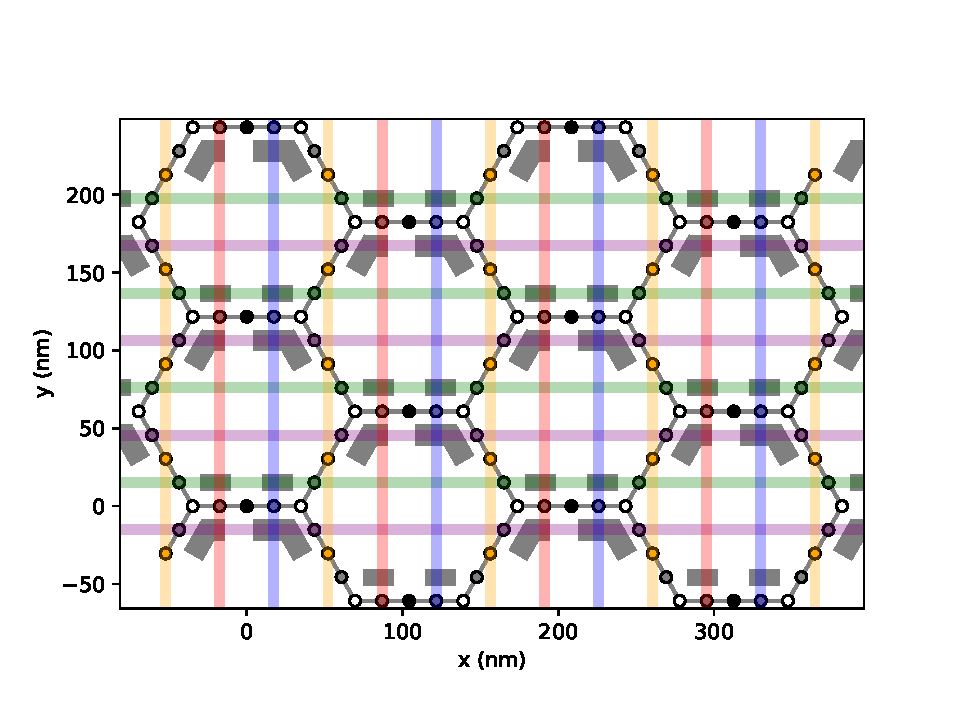
\includegraphics[width=8.15cm]{graphics/ArchitectureDesign/cell_array.pdf}
    \includegraphics[width=8.15cm]{Slides/Slide8.PNG}
    \caption{SET SHAPE IS VERY FLEXIBLE. CAN HAVE WIRES COMING OFF IT.\cite{kranz_exploiting_2020} Heavy-hexagon qubit layout, with coupler qubits shown in grey, and arrangement of wires and SETs overlaid. The entire distance 5 code is shown on the left, while a single unit cell is shown on the right. Data, flag and measure qubits are indicated by yellow, white and black circles respectively, while coupler qubits are grey. Wires of the same colour will be at the same voltage throughout the stabilizer routine (excluding measurement), and these colours will be used throughout when plotting wire voltages to distinguish between the different groups of wires. Wires are arranged so that the role of a given wire does not change as it passes from one unit cell to the next, allowing for entire code to be covered in one round of stabilizer measurements.}
    \label{fig:HH-SiP}
\end{figure}

\subsection{CNOT operation}
Each CNOT can be broken down into 5 steps\cite{hill_exchange-based_2021}. (1) An electron is loaded onto the coupler qubit. (2) The information stored on the nuclear spin is swapped to the electron following well established protocols for nuclear electron spin swapping\cite{morton_solid-state_2008}. (3) The CNOT is performed through application of an EMR sequence designed using GRAPE or machine learning techniques. (4) Qubit information is swapped back to the nucleus. (5) Couplers are unloaded. Here it will be assumed that the cumulative time required for each step involved in the CNOT is $1$ $\mu$s. This can be refined in future by determining and summing the times required for each of the five steps. Determining gate voltage schedules which facilitate the CNOTs involved in the stabilizer measurements amounts to working out the voltages which will load the desired couplers at each step, while keeping all code qubits loaded throughout.

\subsection{Measurement and initialisation}
 Electron spin is read out following established methods for single shot spin readout\cite{morello_single-shot_2010}, whereby source and drain wires of SETs near to the donor being read are tuned such that the source-SET-drain system is in Coulomb blockade only when an electron is present on the donor, and spin-0 electrons alone are able to tunnel out of the donor. A spin-0 measurement is made if a pulse of current is registered in the S and D lines, indicating that the electron has tunnelled out and allowed the SET to exit Coulomb Blockade. If no such pulse is recorded, a 1 is measured. Note that since each S and D line in this design is responsible for readout of multiple qubits, it is vital that every SET which a given source or drain wire intersects be in Coulomb blockade during readout, so that current is blocked until a successful 0 readout occurs.
 
The time taken to perform readout of a single qubit can be understood as the time which the qubit must be left in the readout configuration in order for an energetically allowed tunneling event to occur with high probability. The tunnel rates between SETs and donors is reported somewhat inconsistently in the literature, and is highly dependent on the number of P-donors making up the quantum dot. For now, we assume a time 
\begin{equation}
    t_t = 100\text{ nm}
\end{equation} 
will be sufficient for energetically allowed tunneling to have occurred with high probability. 
 
The time taken to perform readout over the entire code scales with code distance. For a distance $d$ code (where $d$ is odd), the number of rows of measurements which much be performed is $(d+1)/2$.




\subsection{Electron loading/unloading - heuristic approach}
Loading of a given donor is accomplished by raising the Fermi level of a nearby SET such that it becomes energetically favourable for an electron to tunnel from the SET island to the donor. This involves negatively biasing the wires which intersect at the SET island, which causes a build up of electron on the SET island. The wire voltages also affect the Fermi levels of the donors, which facilitates preferential loading and unloading of donors by making their Fermi levels distinguishable from one another.

A heuristic approach to determining voltage configurations is taken in the interest of demonstrating the viability of the design before performing any simulations of the electrostatics underpinning its operation. This is undertaken by considering several distinct voltage levels, and arguing that certain donors will be loaded while others will be unloaded due to differences in their proximities to particular wires.

\begin{figure}
    \centering
    \includegraphics[height=4.8cm]{graphics/fermis.PNG}\hspace{15pt}
    \includegraphics[height=4.8cm]{graphics/readout_diagrams.png}\hspace{10pt}
    \includegraphics[width=1.3cm]{graphics/Vscale2.PNG} 
    \caption{Voltage configurations for measure and flag qubit readout and re-initialisation as required for stabilizer measurements. A positive tilt voltage $V_{t}$ through the gold wire renders the Fermi level of the flag qubits (white) lower than that of the measure qubit (black) indicated by the diagram on the left. The two source-drain configurations correspond to measurement/re-initialisation of measure (left) and flag (right) qubits, with the source wire operating just below the spin-0 electron energy level on the donor to allow readout, while both lines are above the spin-1 level, facilitating re-initialisation. Both configurations are assumed to be in Coulomb blockade when an electron is present on the donor.}
    \label{fig:fermis}
\end{figure}

\subsection{Constraints}
Design constraints which have dictated wire and SET placement are listed below. 
\begin{enumerate}
    \item Gate separation is constrained by the pitch limit, which prohibits placement of the nanowires any nearer than 30 nm from one another.
    \item Qubits must be closely spaced, preferably around $15$ nm apart, to allow for strong exchange interaction. Application of a strain field\cite{hill_exchange-based_2021} may be incorporated to increase this distance up to around $20$ nm.
    \item Wires which are associated with SETs are required to pass much closer to coupler qubits than to code qubits, to ensure that all code qubits can be loaded prior to the loading of any coupler qubits.
    \item Wire layout should allow parallel operation of as many stabilizers as possible. 
\end{enumerate}

\subsection{Assumptions}
\begin{enumerate}
    \item An SET voltage configuration $V_{\text{source}} \ll V_{\text{drain}}\ll 0$ can be employed in which the larger magnitude $V_{\text{source}}$ wire doubles as a control wire, raising the Fermi level of coupler qubits which it passes over, thereby enabling preferential loading (see Figure \ref{fig:X-CNOT}). This relies on the SET island operating at a stable Fermi level in between the levels corresponding to voltages $V_{\text{source}}$ and $V_{\text{drain}}$. 
    
    \item Direct tunneling between wires and qubits is negligible. This is particularly important for readout, when a positive voltage is applied to group 3 wires passing directly over data qubits.
    \item Commuting CNOTs can be performed in parallel. In reality the $\pm 1$ lattice site donor placement imprecision may impose  limitations on parallel operation. This extends to CNOTs which share a qubit, such as CNOTs between qubit pairs [4,5], [3,5], [1,6], and [2,6] shown in figure \ref{fig:X-CNOT}, which are all assumed to be operated in parallel.
\end{enumerate}


\begin{figure}[h]
    \centering
    \includegraphics[height=8.25cm]{graphics/cnot_voltages.pdf}
    \hspace{-15pt}\includegraphics[height=7.05cm]{graphics/tallX.PNG} \vspace{2pt}\newline
    \includegraphics[width=4.4cm]{Slides/Slide9.PNG}
    \includegraphics[width=4.4cm]{Slides/Slide10.PNG}
    \includegraphics[width=4.4cm]{Slides/Slide11.PNG}\hspace{10pt}
    \includegraphics[width=1.15cm]{graphics/Vscale.PNG}
    \caption{X-stabilizer wire voltage schedule is plotted, with upper right unit cell showing the wire corresponding to each colour used in the plot. The routine is broken up into steps (a) - (e). The bottom three diagrams show the state of the unit cell at each step, with loaded couplers coloured red. Each wire has access to four distinct voltage levels plotted as dotted horizontal lines. Note that colour coding in upper graphics is used to identify wires, while colours in bottom strip indicate voltage strength.}
    \label{fig:X-CNOT}
\end{figure}


\subsection{X-stabilizer CNOTs}
The initial configuration has the code qubits loaded and the couplers unloaded, with flag and measure qubits appropriately initialised as shown in Figure \ref{fig:X-CNOT}. The X-stabilizer CNOTs are performed, followed by readout and re-initialisation of measure and flag qubits.

Three voltages, $V_pt$, $V_{p1}$, and $V_{p3}$, are used to show the working of the stabilizer CNOTs, with
\[V_t<V_{p2}<V_{p1}<0.\] 
The gate voltages are offset so that at zero voltage, all qubits are unloaded\cite{hill_surface_2015}. $V_{pt}$ is a plunged tilt voltage used to raise the Fermi levels of coupler qubits which it passes closest to, thereby preventing them from loading. $V_{p2}$ and $V_{p1}$ are plunge voltages, with $V_{p1}$ sufficient to load code qubits, while $V_{p2}$ loads coupler qubits as well. No attempt is made to provide values for these voltages, it is merely claimed that values exist which will facilitate the operation of the design. All CNOTs stabilizer CNOTs across the code are performed in parallel, allowing the operating time to be independent of code distance. Voltage schedule for the X-stabilizer CNOTs is shown in figure \ref{fig:X-CNOT}.





%An SET-coupler tunnel rate of $\sim1$ GHz\cite{extracting-inter-dot-tunnel-couplings} gives characteristic time $t_c = 1\text{ ns}$. We assume tunneling will have occurred with sufficiently probability after 5ns, which we will call the coupler tunnel time $t_{t}=5\text{ ns}$. We assume CNOT timescale is $t_{\otimes}=1 \ \mu\text{s}$ and nuclear spin swap has timescale $t_{\text{SW}}= 100\text{ ns}$.







\subsection{X-stabilizer ancilla readout}
For readout of measure and flag qubits, a positive tilt voltage $V_t$ is used to ensure that the measure qubits unload before the flag qubits (see figure \ref{fig:fermis}). Readout occurs at voltages between $V_{p1}$ and zero, where $V_{p1}$ is the same plunge voltage introduced in the CNOTs section. We must therefore consider additional voltages $V_b,V_w$ with 
\begin{equation}
    V_{p1}<V_b<V_w<0<V_t,
\end{equation}
with $V_b$ and $V_w$ representing the voltages above which a spin up electron residing on the measure and flag qubits respectively will be able to tunnel out. 

Re-initialisation is assumed to have the same time requirement as readout, but can be performed across the entire code simultaneously. It is assumed that flag and measure qubits must be re-initialised in separate steps as the flag qubits are initialised to $\ket{0}$, while the measure qubit is inialised to $\ket{+}$. The measure qubit can be initialised into the $\ket{+}$ state by performing a global Hadamard before and after loading of the measure qubit electron. The time taken to perform this Hadamard is ignored.


\begin{figure}
    \centering
    \includegraphics[width=11.5cm]{graphics/tall_measure.pdf}
    \hspace{-20pt}
    \includegraphics[width=5cm]{graphics/yikespv.png}
    \caption{X-stabilizer measurement and re-initialisation voltage schedule. The two voltage source-SET-drain configurations described in figure \ref{fig:fermis} are utilised for measure and flag qubit readout. Indicated voltages $V_b$ and $V_w$ are the gate voltages beyond which a spin-$0$ electron can tunnel out of the measure qubit or flag qubit respectively. Each step is as follows:  (1)-(3): flag qubit readout. (4)-(6): measure qubit readout. (7): Measure qubit re-initialisation. (8): Flag qubit re-initialisation. The vertical wires plotted in red and blue act as the drain gates, operating just below the dotted lines, which not allow tunneling out of spin-$0$ (or spin-$1$) electrons. The purple and green horizontal wires act as the source gates, operating just above the dotted lines during loading and readout, which allows spin-$0$ electrons to tunnel out of donors and spin-$1$ to tunnel in. Three sets of source wires are plotted, as readout occurs in three rows for the distance 5 code. Each of the source wires must remain just below the appropriate dotted line when it is not its turn for read out, maintaining a non-readout Coulomb blockaded configuration. Graphics (1), (2), (3), show gate voltages across the distance 5 code in steps (1), (2) and (3), illustrating the top to bottom measurement sweep which is performed. Thick purple wires are at a voltage just above $V_b$, thin purple just below.}
    \label{fig:my_label}
\end{figure}

For a distance 5 code, there are 5 groups of CNOTs, followed by 3 rounds of measurements for each the measure and the flag qubits (giving 6 in total), followed by re-initialisation of flag and measure qubits. Assuming CNOT time of $1\ \mu$s and tunnel time of 100 ns total X-stabilizer time
\begin{equation*}
    T_X = 5.8\ \mu\text{s}.
\end{equation*}

\subsection{Z-stabilizer}
The Z-stabilizer shown in figure \ref{fig:Zstab} is simple in comparison to the X-stabilizer, with its steps forming a subset of the steps involved in the X-stabilizer. As such, details of its operation are omitted. There is one round of CNOTs, followed by 3 rows of flag qubit measurements, and re-initialisation of flag qubits. The total time taken given previous CNOT and tunneling time assumptions is
\begin{equation}
    T_Z = 1.4\ \mu\text{s}.
\end{equation}

We thus arrive at a total time for the completion of one round of stabilizer measurements,
\begin{equation}
    T = 7.2\ \mu\text{s}.
\end{equation}


\begin{figure}
    \centering
    \includegraphics[width=10cm]{graphics/Zstab.PNG}
    \caption{Z-stabilizer routine.}
    \label{fig:Zstab}
\end{figure}



\end{document}